\chapter{Aproximación numérica utilizando Monte Carlo}
{\label{cap.singular}}

En el presenta capítulo se desarrollara un formalismo para calcular la acción efectiva, y por lo tanto la energía de casimir.
Se aplicaran estos resultados a un campo confinado entre dos placas paralelas en el vacío sin interacción.

\section{La acción efectiva}



Dado un lagrangiano de la forma


\begin{equation}
\mathscr{L} = \frac{1}{2} \partial _{\mu} \phi  \partial _{\mu} \phi +
	\frac{m^2}{2} \phi ^2  + \frac{1}{2} V(x) \phi ^2
	\, ,
\end{equation}
en la ausencia de campos o acoplamientos la acción efectiva puede ser escrita como


\begin{align}
\Gamma \left[ V \right] =&
  \frac{1}{2} Tr Ln \frac{- \partial ^2 + m ^2 + V(x)}{- \partial ^2 + m ^2} \\ 
 =& - \frac{1}{2} \int _{\frac{1}{\Lambda ^2}} ^{\infty} \frac{dT}{T} \int dx dt \left[ \left< x | e ^{-T (- \partial ^2 + m ^2 + V(x))} | x  \right> \right] \, ,
\label{cap4.accion_efecitva}
\end{align}


%

donde en la segunda integral se puede interpretar el elemento de matriz como la amplitud de transición a tiempo propio $T$, por lo tanto se puede introducir la representación de linea de mundo dada por.


\begin{align}
& \int dx  dt \left< x | e ^{-T (- \partial ^2 + m ^2 + V(x))} | x  \right> = \\
& \int dx  dt \, 
\mathcal{N}  \int _{x(0) = x(T)} \mathscr D x e ^{- \int _0 ^T d \tau  \frac{\dot{x} ^2}{4} - V(x + x( \tau )) }
\nonumber
\, ,
\label{eq.definicion_ensamble}
\end{align}
dado que en \eqref{cap4.accion_efecitva} la amplitud de transición se calcula entre dos puntos coincidentes, la integral de caminos debe ser calculada sobre lineas de mundo cerradas $x(0) = x(T)$, la constante de normalización $\mathcal{N}$ queda determinada por el límite de cero potencial.


Esta integral de caminos puede ser interpretada como el valor medio en un ensamble de lineas de mundo con distribución de velocidad gaussiana
\begin{equation}
\mathcal{N} 
\int _{x(0) = x(T)} \mathscr D x e ^{- \int _0 ^T d \tau \frac{\dot{x} ^2}{4} - V(x + x( \tau )) } =
\frac{1}{4 \pi T} \left<  e ^{- \int _0 ^T dt   V(x + x(t)) }  \right> _{x}
\, ,
\label{eq_valores_medio}
\end{equation}

como último paso se introducirán loops unitarios, que son lineas de mundo parametrizadas con un tiempo propio $t \in [0,1]$

\begin{equation}
y _{\mu} (t) = \frac{1}{\sqrt{T}} x _{\mu} (T t)
\Longrightarrow
\int _{0} ^{T} d \tau \, \dot{x ^2 ( \tau)} = \int _{0} ^{1} dt \, \dot{y ^2 ( t)}
\, .
\label{def.loop_unitarios}
\end{equation}

Utilizando \eqref{def.loop_unitarios} y  \eqref{eq_valores_medio} en \eqref{cap4.accion_efecitva} se obtiene una representación de la acción efectiva dada por

\begin{equation}
\Gamma \left[ V \right] = 
\left<
-  \frac{1}{8 \pi}
\int _{\frac{1}{\Lambda}} ^{\infty} \frac{dT}{T^ {2}} e ^{- m^2 T}
\int dx \left( W _v [ y(t); x] - 1\right)
\right> _{y} 
 ,
\label{accion_efectiva_path_integral}
\end{equation}


donde
\begin{equation}
W _v [ y(t); x] = exp \left[ -T \int _{0} ^{1} dt V( x + \sqrt{T} y(t)) \right]
 , 
\label{eq.definicion_w}
\end{equation}
Para calcular el valor medio \eqref{accion_efectiva_path_integral} hay diversas técnicas enumeradas en \cite{Gies_2003} en particular se seguirá el metodo realizado en \cite{Franchino_Vi_as_2019}, en este trabajo se utilizará la diagonalización explícita de la acción "v loops".


%Donde surge el vinculo que los loops tengan distribución de velocidad gaussiana
%\begin{equation}
%P[{y(t)}] = \delta \left(  \int _{0} ^{1} y(t) \right) exp \left(  -\frac{1}{4} \int _{0} ^{1} dt \dot{y} ^2 \right)
%\end{equation}

\section{Algoritmo v loops}


Dados dos puntos inicial y final $ y_0$, $ y_N$ respectivamente, el algoritmo se basa en crear un ensamble de lineas que unan estos dos puntos siguiendo una distribución de velocidad gaussiana.
 


\begin{equation}
\mathcal{N} \int _{y_0} ^{y_N} \mathcal{D} y 
e^{-\frac{N}{4} S _{W} [y]} :=
\mathcal{N} \int \prod _{j=1} ^{N-1} d ^{D} y _{j} e^{- \frac{N}{4} \sum _{i=1} ^{N} ( y _i - y _{i-1} )^2 } ,
\label{eq.definicion_accion_discreta}
\end{equation}

el objetivo es realizar un sistema de cambios lineales de manera que la distribución de probabilidad se vuelve puramente guassiana, con este fin se completan cuadrados para la variable $ y_1$


\begin{equation}
S _{W} = 	2 \left( y _1 - \frac{y_0 + y_2}{2} \right) ^2 + 
			\frac{1}{2} \left( y ^2 _2 + y _0 ^2 \right)   -
			y _0 y_2 +
			\sum _{i = 3} ^{N} (y _i - y _{i-1}) ^2 
\, ,
\end{equation}

donde existe un solo término que contiene $y_0$, se define entonces la variable

\begin{equation}
z _1 := y_1 - \frac{y _0  + y_2 }{2} ,
\end{equation}
realizando el mismo procedimiento para la variable $y_1$ se obtiene


\begin{equation}
S _W = 2 z_1 ^2 +
		\frac{3}{2} \left( y _2 - \frac{y _0 + 2 y_3}{3} \right) ^2 +
		\frac{1}{3} \left( y _3 ^2 + y _0 ^2 \right) -
		\frac{2}{3} y_0 y_3 +
		\sum _{i = 4} ^{N} (y _i - y _{i-1}) ^2 
		,
\end{equation}
resultando la forma cuadrática
\begin{equation}
z _2 := y_2 - \frac{y _0  + 2 y_3 }{3} ,
\end{equation}
la expresión general luego de completar cuadrados en la variable $y_i$ queda determinada por 
\begin{equation}
a _i y _i ^2 - 2 y_i ( y _{i+1} + b _i y_0 ) =
a _i \left( y _i - \frac{y _{i+1} + b_i y_0}{a_i} \right) ^2 -
\frac{\left( y _{i+1} + b_i y_0 \right) ^2}{a _i}
\, .
\end{equation}


Donde los coeficientes $a_i$ y $b_i$ están dados por el sistema de ecuaciones recurrentes

\[ 
f   ( i t ,\beta )=
\begin{cases} 
	  a_{i+1} = 2 - \frac{1}{a_i},  \, a _1 = 2
\\
	  	  b_{i+1} = \frac{b _i}{a _i},  \, b _1 = 1
   \end{cases}   
\] 

conde la solución está dada por
\begin{equation}
a _1 = \frac{i+1}{i} ; \, b_i = \frac{1}{i} ,
\end{equation}

por lo tanto la forma general de las variables $z _i$ queda definida por
\begin{equation}
z _i = y _i - \frac{y_0}{i+1} - \frac{i}{i+1} y _{i+1} ,
\end{equation}

reescribiendo la acción con estas nuevas variables, el exponente queda diagonalizado de la forma

\begin{equation}
S _{W}  = \sum _{i = 1} ^{N-1} \frac{i +1}{i} z _i ^2 + c y _0 ^2 + d y _N ^2
, 
\end{equation}
los valores $c$ y $d$ no son importantes ya que son constantes que se cancelarán con la correspondiente normalización.
En resumen el algoritmo de los v loops, dados $N-1$ puntos intermedios queda determinado por 
\begin{enumerate}
\item Generar $N-1$ numeros $w_i$ que estén distribuidos de acuerdo a la distribución de velocidades $e^{- w _{i} ^2}$
\item normalizar las variables $w _i$ para obtener las variables auxiliares $z _i$
	\begin{equation}
	z _i = \sqrt{\frac{4}{N}} \sqrt{\frac{i}{i+1}} w _i
	\end{equation}

\item Una vez obtenidos los puntos $ z_i$ se calculan los puntos $ y_i$ por medio de la formula recursiva
	\begin{equation}
	y _i = z _i + \frac{1}{i+1} y_0 + \frac{i}{i+1} y _{i+1} ,
	\end{equation}
\end{enumerate}
en el caso que $y_0 = y _N$ se obtienen loops cerrados de $N-1$ puntos puntos intermedios.
En la figura \ref{fig:ejemplo_loops} se puede observar un ejemplo de la generación 5 loops cerrados con este algoritmo donde $N=31$.


\section{Test del algoritmo de los v loops}


Considerese la acción en un espacio $N-1$ dimensional definida en \eqref{eq.definicion_accion_discreta} el cual genera una distribución de probabilidad dada por 
\begin{equation}
P [y] = \mathcal{N} e^{-S _{W} [y]}
\, .
\end{equation}
El valor medio de la acción está dado por
\begin{equation}
\left< S _W \right> = 
\mathcal{N} \int dy _1 ... dy _{N-1} S _w [y] e^{-S _{W} [y]} =
\frac{1}{2} (N-1) D + \frac{1}{4} \Delta y ^2 
\,
\end{equation}
en la figura \ref{fig:convergencia_loops} se puede ver como al aumentar el número de loops la aproximación numérica tiende el valor de la acción. \\



La distribución de probabilidad que genera esta acción está dada por
\begin{align}
\mathcal{P} [S _W] &=  \mathcal{N} \int d y_1 \dotsb d y_{N-1} \delta \left( S_W - S_{W'}  \right) e ^{S_W}  \\
&=
 \mathcal{N} \left(  S' _W - S_{class} \right) ^{-1 + \frac{(N+1) D}{2}}
e ^{-\left( S' _W - S_{class} \right)}
\theta \left( S ' _W - S _{class} \right)
\, ,
\nonumber
\end{align}
donde la acción clásica está dada por
\begin{equation}
S _{class} = \frac{\Delta y ^2}{ 4}
\, .
\end{equation}
En la figura \ref{fig:distribucion_accion_cap4} se puede comprar el resultado numérico de la simulación con el resultado analítico 




\begin{figure}
    \centering
    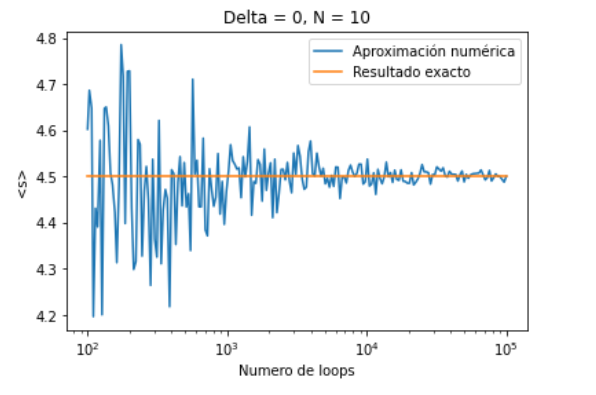
\includegraphics[scale=0.6]{loops_accion.pdf}
    \caption{Aquí se puede ver como al aumentar el número de loops el resultado converge al valor analítico de la acción, aquí se gráfico solamente el valor medio y no su error. }
    \label{fig:convergencia_loops}
\end{figure}

\begin{figure}
    \centering
    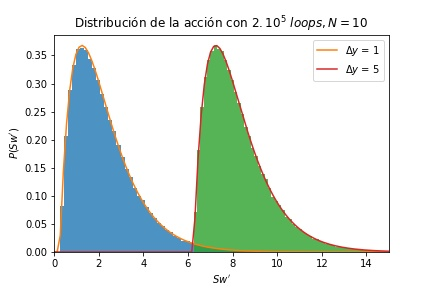
\includegraphics[scale=0.6]{distribucion_accion.jpg}
    \caption{En esta figura se puede observar como la distribución los datos obtenidos a partir del algoritmo de los v loops convergen a la distribución de la acción calculada de manera analítica}
    \label{fig:distribucion_accion_cap4}
\end{figure}



\section{Cálculo numérico de la energía de casimir}


En esta sección se utilizará el algoritmo de los v loops para calcular la acción efectiva en un potencial de placas paralelas en el límite de condiciones Dirichlet dado por

\begin{equation}
V(x) = \lim _{\lambda \rightarrow \infty} \lambda \left( \delta (x) + \delta ( x - a) \right)
\, .
\label{eq.definicion_potencial_D}
\end{equation}

Utilizando el potencial \eqref{eq.definicion_potencial_D} en \eqref{eq.definicion_w} el efecto neto es obtener una función escalón, donde el valor es $1$ si para un dado valor de $x$ y $T$ el loop penetra ambas superficies y cero en el caso contrario. \\


Dado un loop $y = y(t)$ las condiciones para que toque ambas placas están dadas por

\begin{align}
\label{condiciones}
\sqrt{T} y_{max} + x & \geq a \\
\sqrt{T} y_{min} + x & \leq 0 \, ,
\nonumber
\end{align}
donde 
\begin{align*}
y_{max}  &= max(y(t)) \\
y_{min}  &= min(y(t)) \, .
\end{align*}




\begin{figure}
    \centering
    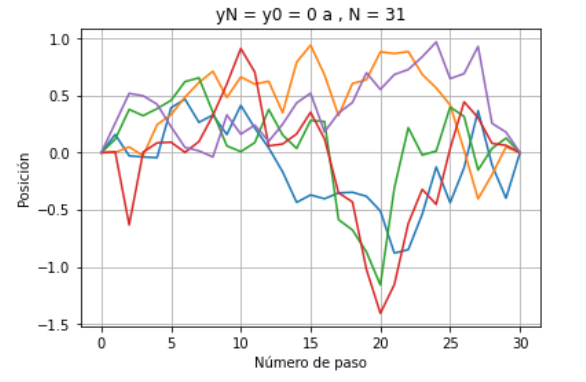
\includegraphics[scale=0.6]{ejemplo_loops.pdf}
    \caption{Muestreo de 5 loops generados para calcular la integral}
    \label{fig:ejemplo_loops}
\end{figure}



Lo cual conduce a una acción acción efectiva dada por

\begin{align}
\label{ec1.accion_efectiva}
\Gamma \left[ V \right] = 
 \Bigg<
&- \frac{\Delta y}{8 \pi}
	\left(
		\frac{2 \Delta y e^{-\frac{(m a)^2}{\Delta y ^2}}}{a}
		-2 m \Gamma \left( \frac{1}{2}, \frac{(m a)^2}{\Delta y ^2} \right)
	\right) \\
	&-  \frac{a}{8 \pi}
	\left(
		\frac{\Delta y ^2 e^{-\frac{m^2 a^2}{\Delta y^2}}}{a^2} -
		m^2 \Gamma \left( 0, \frac{m^2 a^2}{\Delta y ^2} \right)
	\right)	
\Bigg> _{y} 
\, ,
\nonumber
\end{align}

donde la función gamma incompleta está definida por
\begin{equation*}
\Gamma (a, z) = \int _{z} ^{\infty} t^{a-1} e ^{-t} dt
\, .
\end{equation*}

A partir de aquí se puede obtener la energía de vacío tomando la derivada  $\partial a$, lo que resulta en una Fuerza de casimir dada por
\begin{equation}
F (m,a) = 
\frac{m^2 \Gamma \left( 0 , \frac{a ^2 m^2}{\Delta y^2} \right)}{8 \pi}
- \frac{\Delta y^2 \, e ^ {-\frac{a ^2 m^2}{\Delta y^2}}}{8 \pi a^2 } 
\, ,
\label{eq.fuerza.casimir.numerica}
\end{equation}
lo cual en la figura \eqref{fig:fuerza_Casimir_masa} está comparado con el valor exacto dado por
\begin{equation}
F _{exacto} (m,a) = - \int _{m} ^{ \infty } \frac{dt}{\pi} \frac{t^2}{\sqrt{t^2 -m^2}(e^{2 t a} -1)}
\, .
\end{equation}


En el límite de masa cero la ecuación \eqref{eq.fuerza.casimir.numerica}  toma la conocida dependencia con $a^{-2}$, que corresponde a la Fuerza de Casimir en $D = 1+1$
\begin{align}
\lim _{m \rightarrow 0} F(m,a) = - \frac{\Delta y^2}{8 \pi a^2} \\
F _{exacto} (a) = - \frac{\pi}{24 a^2}
\, ,
\end{align}
en la tabla \ref{table:1} y en la figura \ref{fig:convergencia_loops} el valor calculado con el resultado exacto al variar el número de loops y la cantidad de puntos intermedios.




\begin{figure}
    \centering
    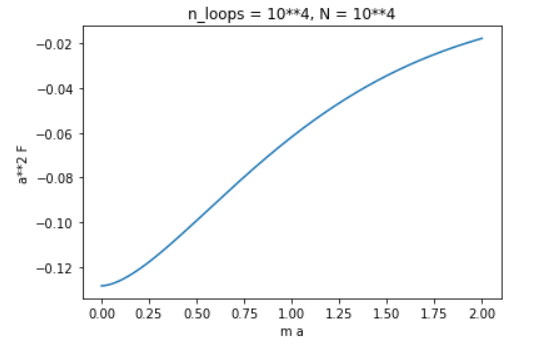
\includegraphics[scale=0.6]{fuerza_casimir_masa_linea.pdf}
    \caption{En esta figura se puede ver la dependencia de la Fuerza de Casimir $a^2 F(m,a)$ en función de $m a$, el error es la desviación estándar muestral, se utilizaron 1.000 loops y 1.000 puntos intermedios.}
    \label{fig:fuerza_Casimir_masa}
\end{figure}


\begin{figure}
    \centering
    \includegraphics[scale=0.6]{convergencia.pdf}
    \caption{En esta figura se puede observar como al aumentar el número de puntos por loops se reduce el error sistematico debido a la discretización de los loops.}
    \label{fig:convergencia_loops}
\end{figure}



\begin{table}
\begin{center}
 \begin{tabular}{|| c c c||} 
 \hline \\ 
 num. loops & N & $\frac{ \Delta F}{F}$ \\ [0.5ex] 
 \hline\hline
  10.000 & 10.000& 0.013 \\ 
 \hline
  1.000 & 10.000 & 0.024 \\
 \hline
  100 & 10.000 & 0.037\\
 \hline
  10.000 & 1.000 & 0.05 \\
 \hline
  1.000 & 1.000 & 0.058 \\ 
 \hline
   100 & 1.000 & 0.10 \\
 \hline
  10.000 & 1000 & 0.17\\
 \hline
  1.000 & 100 & 0.18 \\
 \hline
   100 & 100 & 0.20 \\ [1ex] 
 \hline
\end{tabular}
\end{center}
\caption{En esta tabla se puede ver como al aumentar el numero de loops y el número de puntos intermedios, el cálculo converge al resultado teórico.}
\label{table:1}
\end{table}
